%*******10********20********30********40********50********60********70********80
\chap{Background Theory}

What the reader needs to know in order to understand the rest of the report. Examiners like to know that you have done some background research and that you know what else has been done in the field (where relevant). Try to include some references.
    Related work (if you know of any)
    What problem are you solving?
    Why are you solving it?
    How does this relate to other work in this area?
    What work does it build on?
    
\section{Agile Software Development}

\newpage

\section{Ruby on Rails} 
Ruby on Rails, or simply Rails, is a server-side web application framework written in Ruby under the MIT License. Rails is a model–view–controller (MVC) framework, providing default structures for a database, a web service, and web pages. \cite{wiki:RoR}

\begin{figure}[H]
	\centering
    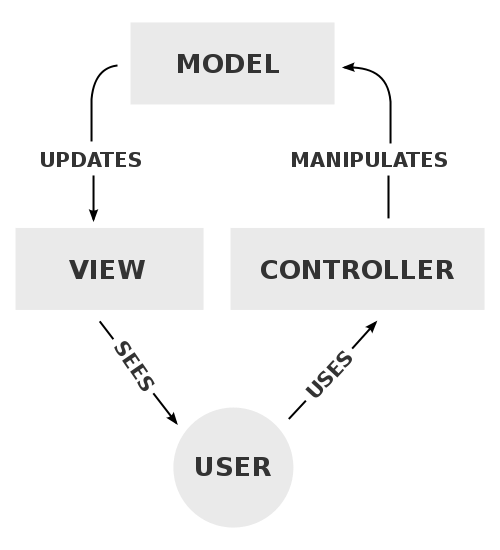
\includegraphics[trim={0 0 0 0},clip,width=0.5\textwidth]{Files/MVC.png}
    \caption{Diagram of interactions within the MVC pattern.\\ \textbf{Source:} https://en.wikipedia.org/wiki/Model-view-controller}
    \label{fig: MVC}
\end{figure}




\textbf{The Model:}
\vspace{-5mm}
\begin{itemize}
 \setlength{\itemsep}{-5pt}
\item Contains data for the application (often linked to a database)
\item Contains state of the application (e.g. what orders a customer has)
\item  Contains all business logic
\item Notifies the View of state changes (** not true of ROR, see below)
\item No knowledge of user interfaces, so it can be reused
\end{itemize}

\textbf{The View:}
\vspace{-5mm}
\begin{itemize}
 \setlength{\itemsep}{-5pt}
\item Generates the user interface which presents data to the user
\item Passive, i.e. doesn’t do any processing
\item Views work is done once the data is displayed to the user.
\item Many views can access the same model for different reasons
\end{itemize}

\textbf{The Controller:}
\vspace{-5mm}
\begin{itemize}
 \setlength{\itemsep}{-5pt}
\item Receive events from the outside world (usually through views)
\item Interact with the model
\item Displays the appropriate view to the user
\end{itemize}

https://stackoverflow.com/questions/1931335/what-is-mvc-in-ruby-on-rails




